% NeuroCam manual - Cameras
% Written by Christopher Thomas.
% Copyright (c) 2021 by Vanderbilt University. This work is released under
% the Creative Commons Attribution-ShareAlike 4.0 International License.

\chapter{Cameras}
\label{cameras}

\section*{Camera Selection}

The NeuroCam system is compatible with any UVC-compliant USB camera capable
of producing MJPEG output. That said, there are several additional qualities
that cameras \textit{should} possess:

\begin{itemize}
\item The camera should support 1280x720 or better resolution at 30~fps.
\item The camera should either not have an infrared filter or should have an
infrared filter than can be easily removed (not bonded to the sensor die).
\item The camera should request only the USB bandwidth it needs, rather than
attempting to request all USB bandwidth.
\end{itemize}

The Logitech C920 webcam satisfies these requirements and was used for the
prototype systems. Infrared filter removal with this camera is described in
Chapter \ref{c920}.

\section*{Infrared LED Mounting}

An infrared LED is bonded to each camera to allow individual camera feeds
to be synchronized with high accuracy via strobe flashes. This LED should
not obstruct the scene, but should still be within the camera's field of
view for all video resolutions of interest.

The recommended procedure for mounting LEDs is to set up a video feed from
the camera, apply cyanoacrylate glue (``super glue'') to the camera case,
hold the LED mounting rod in position until the glue sets (using the video
feed to guide placement), and then to apply two-part epoxy for a more
permanent bond.

For the Logitech C920, positioning the LED in the upper left corner of the
field of view when using a 4:3 resolution guarantees that it is visible in
all video modes (4:3 and 16:9).

The parts needed to add LEDs to each camera are as follows:

\begin{tabular}{llll}\hline
Qty & Description & Manuf. p/n & Digikey p/n \\
\hline
1 & NIR LED 940nm & SLED-56-16639 & SLED-56-16639-ND \\
1 & BNC female to wire & BU-P4969 & 314-1190-ND \\
\hline
\end{tabular}

Mechanical details for mounting LEDs to Logitech C920 cameras are shown
below:

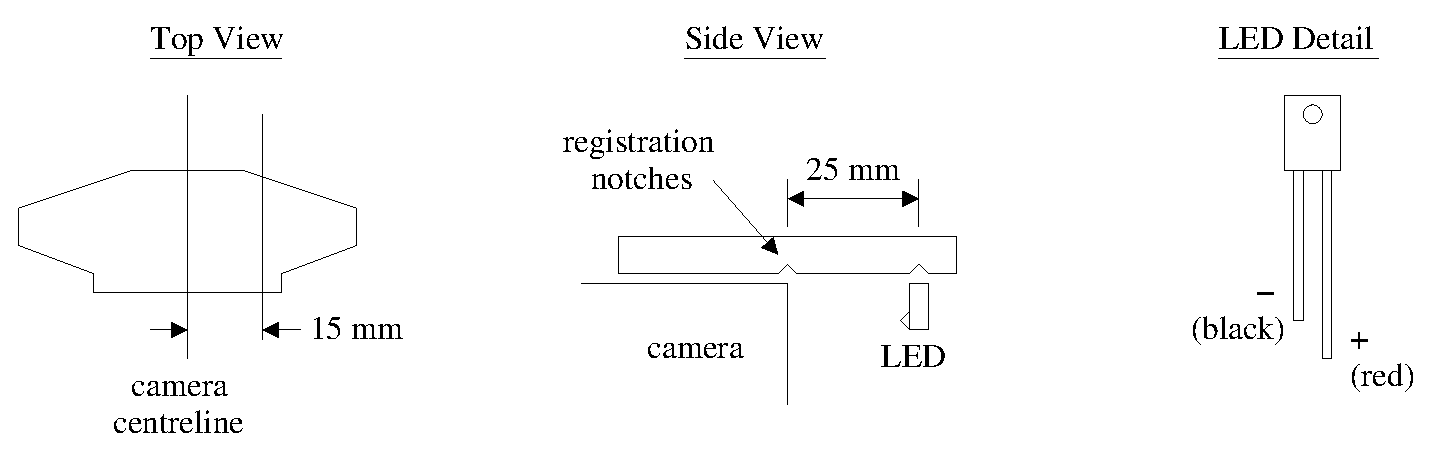
\includegraphics[width=0.9\textwidth]{figs/maint-led-920.pdf}

The result is shown below:
\begin{center}
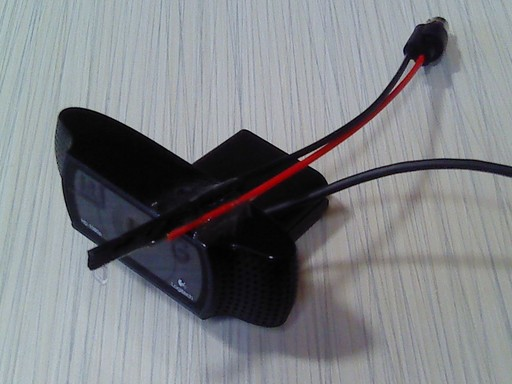
\includegraphics[height=3in]{pics-cam/c920-led.jpg}
\end{center}

%
% This is the end of the file.
